\documentclass[14pt,a4paper]{extarticle}
\usepackage[T1]{fontenc}
\usepackage[utf8]{inputenc}
\usepackage[scaled]{helvet}
\renewcommand{\familydefault}{\sfdefault}
\usepackage{amsmath}
\usepackage{sansmath}
\sansmath
\usepackage[a4paper,margin=2cm]{geometry}
\usepackage{tikz}
\usetikzlibrary{angles,quotes,patterns}
\usepackage{array}
\pagestyle{empty}
% Zweite Seite: 5-mm-Kästchen, 1 cm Rand
\newcommand{\kaestchen}{\newpage\null\begin{tikzpicture}[remember picture,overlay]
\begin{scope}[shift={(current page.south west)}]\draw[step=5mm, black!45, line width=0.3pt] (1cm,1cm) grid (20cm,28.5cm);\draw[black!45, line width=0.3pt] (1cm,1cm) rectangle (20cm,28.5cm);\end{scope}
\end{tikzpicture}}
\setlength{\parindent}{0pt}
\hyphenpenalty=10000

% Nur Schwarz und Grau, die Blätter werden schwarz-weiß kopiert.
% Merkblock: Begriff und Text links, Zeichnung rechts.
\newcommand{\bl}{0.5}
\newcommand{\block}[3]{%
\begin{minipage}[c]{\bl\textwidth}\raggedright{\Large\bfseries #1\par}\medskip #2\end{minipage}\hfill
\begin{minipage}[c]{\dimexpr0.97\textwidth-\bl\textwidth\relax}\centering #3\end{minipage}\par}

% Die Tabelle beim Wechselwinkel braucht etwas mehr Breite.
\renewcommand{\bl}{0.58}
% Zwei Parallelen g und h, geschnitten von f. Winkelflächen werden als Argument übergeben.
\newcommand{\parfig}[1]{%
\begin{tikzpicture}[scale=1.4]
  \coordinate (G) at (0.866,1.5); \coordinate (H) at (-0.866,-1.5);
  #1
  \draw[thick] (-2.1,1.5) -- (2.1,1.5) node[right] {$g$};
  \draw[thick] (-2.1,-1.5) -- (2.1,-1.5) node[right] {$h$};
  \draw[thick] (-1.5,-2.6) -- (1.5,2.6) node[above right] {$f$};
\end{tikzpicture}}
\newcommand{\wk}[5]{\fill[#4] (#1) -- ++(#2:0.6) arc (#2:#3:0.6) -- cycle; \node at ([shift={({(#2+#3)/2}:0.98)}]#1) {\large$#5$};}

\begin{document}

{\LARGE\bfseries Stufenwinkel und Wechselwinkel\par}
\vspace{0.9cm}

\block{Stufenwinkel}{%
Die Gerade $f$ schneidet die Parallelen $g$ und $h$. Stufenwinkel liegen an beiden Kreuzungen an der gleichen Stelle. Sie sind gleich groß.
\[\alpha_1 = \alpha_2\]
Umgekehrt: Sind Stufenwinkel gleich groß, dann sind $g$ und $h$ parallel.}{%
\parfig{\wk{G}{0}{60}{gray!40}{\alpha_1}\wk{H}{0}{60}{gray!40}{\alpha_2}}}

\vspace{1cm}

\block{Wechselwinkel}{%
Wechselwinkel liegen auf verschiedenen Seiten von $f$ und an verschiedenen Parallelen. Sie sind gleich groß.
\[\alpha_1 = \gamma_2\]
Kennst du einen Winkel, kannst du alle acht angeben.\par\medskip
Beispiel: $\alpha_1 = 60^\circ$\par\smallskip
\begin{tabular}{@{}ll@{}}
$\gamma_1 = 60^\circ$ & Scheitelwinkel zu $\alpha_1$\\[2pt]
$\alpha_2 = 60^\circ$ & Stufenwinkel zu $\alpha_1$\\[2pt]
$\gamma_2 = 60^\circ$ & Wechselwinkel zu $\alpha_1$\\[2pt]
$\beta_1 = 180^\circ - 60^\circ = 120^\circ$ & Nebenwinkel zu $\alpha_1$
\end{tabular}}{%
\parfig{\wk{G}{0}{60}{gray!40}{\alpha_1}\wk{G}{180}{240}{gray!20}{\gamma_1}\wk{G}{60}{180}{pattern=north east lines, pattern color=gray}{\beta_1}\wk{H}{0}{60}{gray!20}{\alpha_2}\wk{H}{180}{240}{gray!40}{\gamma_2}}}

\vspace{1cm}

{\Large\bfseries Aufgaben im Heft\par}
\medskip
Buch S.\,49 Nr.\,6, 7, 8, 9, 10, 11\par\smallskip
Buch S.\,50 Nr.\,7, 8, 9, 10, 11

\kaestchen
\end{document}
